\documentclass[aspectratio=169, handout]{beamer}

%\usepackage[table]{xcolor}
\mode<presentation> {
\setbeamercovered{transparent}
  \usetheme{Boadilla}

\renewcommand{\familydefault}{cmss}
\usepackage{bm}
\usepackage{listings}
\useinnertheme{rectangles}
}
\usepackage{amsmath}
\usepackage{bbold}
\usepackage{tcolorbox}
\setbeamercolor{normal text}{fg=black}
\setbeamercolor{structure}{fg= blue}
\definecolor{trial}{cmyk}{1,0,0, 0}
\definecolor{trial2}{cmyk}{0.00,0,1, 0}
\definecolor{darkgreen}{rgb}{0,.4, 0.1}
\definecolor{darkpurple}{rgb}{0.4, 0, 0.6}
\usepackage{array}
\beamertemplatesolidbackgroundcolor{white}  \setbeamercolor{alerted
text}{fg=darkpurple}
\setbeamertemplate{caption}[numbered]\newcounter{mylastframe}

\font\domino=domino
\def\die#1{{\domino#1}}
\usepackage{tikz}
\usetikzlibrary{arrows}
\usepackage{colortbl}

\renewcommand{\familydefault}{cmss}

\usepackage{tikz}
\usepackage{lipsum}
\usepackage{booktabs}

\lstset{%
  language=R,
  basicstyle=\ttfamily\small,
  keywordstyle=\color{blue},
  commentstyle=\color{darkgreen},
  stringstyle=\color{darkpurple},
  showstringspaces=false,
  breaklines=true,
  frame=single,
  backgroundcolor=\color{gray!10}
}

 \newenvironment{changemargin}[3]{%
 \begin{list}{}{%
 \setlength{\topsep}{0pt}%
 \setlength{\leftmargin}{#1}%
 \setlength{\rightmargin}{#2}%
 \setlength{\topmargin}{#3}%
 \setlength{\listparindent}{\parindent}%
 \setlength{\itemindent}{\parindent}%
 \setlength{\parsep}{\parskip}%
 }%
\item[]}{\end{list}}
\usetikzlibrary{arrows}
\usetikzlibrary{arrows.meta, positioning}
\usepackage{pgfplots}
\pgfplotsset{compat=1.17}
\usecolortheme{lily}

\newtheorem{com}{Comment}
\newtheorem{lem} {Lemma}
\newtheorem{prop}{Proposition}
\newtheorem{condition}{Condition}
\newtheorem{thm}{Theorem}
\newtheorem{defn}{Definition}
\newtheorem{cor}{Corollary}
\newtheorem{obs}{Observation}
 \numberwithin{equation}{section}

\makeatletter
\def\beamerorig@set@color{%
  \pdfliteral{\current@color}%
  \aftergroup\reset@color
}
\def\beamerorig@reset@color{\pdfliteral{\current@color}}
\makeatother
\setbeamertemplate{navigation symbols}{}

\useoutertheme{miniframes}
\title[PLSC 30700]{Linear Models Lecture 13: Instrumental Variables}

\author{Robert Gulotty}
\institute[Chicago]{University of Chicago}
\vspace{0.3in}


\begin{document}

\begin{frame}
\maketitle
\end{frame}

%%%%%%%%%%%%%%%%%%%%%%%%%%%%%%%%%%%%%%%%%%%%%%%%%%%
\section{Endogeneity}
%%%%%%%%%%%%%%%%%%%%%%%%%%%%%%%%%%%%%%%%%%%%%%%%%%%

\begin{frame}{Structural vs.\ Projection Parameters}
\begin{itemize}
\item Recall from our earlier lectures: OLS estimates the \textbf{best linear predictor} (projection).
\item A \textbf{structural model} posits a causal data-generating process:
$$Y = \bm{x}'\beta + e$$
\item We can always define a projection: $\beta^*=(\mathbb{E}[\bm{x}\bm{x}'])^{-1}\mathbb{E}[\bm{x}Y]$, with $\mathbb{E}[\bm{x}e^*]=0$.
\item When $\mathbb{E}[\bm{x}e]\neq 0$:
\begin{align*}
\beta^*&=\beta+(\mathbb{E}[\bm{x}\bm{x}'])^{-1}\mathbb{E}[\bm{x}e]\neq \beta
\end{align*}
\item OLS is \alert{inconsistent} for the structural parameter:  $\hat{\beta}\xrightarrow{p}\beta^*\neq\beta$.
\item We call $\bm{x}$ \textbf{endogenous} when this occurs.
\end{itemize}
\end{frame}


%%%%%%%%%%%%%%%%%%%%%%%%%%%%%%%%%%%%%%%%%%%%%%%%%%%
\subsection{Measurement Error}
%%%%%%%%%%%%%%%%%%%%%%%%%%%%%%%%%%%%%%%%%%%%%%%%%%%

\begin{frame}{Endogeneity Source 1: Measurement Error}
\begin{itemize}
\item The true structural model is $\mathbb{E}[Y\mid \bm{z}]=\bm{z}'\beta$, but we don't observe $\bm{z}$.
\item Our measured variables: $\bm{x}=\bm{z}+\bm{u}$, where $\bm{u}$ is measurement error.
\item Assumptions on the error:
\begin{itemize}
\item $\text{plim}\;\frac{\bm{z}'\bm{u}}{n}=0$: measurement error uncorrelated with truth
\item $\text{plim}\;\frac{e'\bm{u}}{n}=0$: measurement error uncorrelated with structural disturbance
\end{itemize}
\item \textbf{Political science examples:}
\begin{itemize}
\item Survey-reported ideology (ANES self-placement on liberal--conservative scale)
\item GDP in developing countries used in aid allocation studies
\item Self-reported voter turnout (overreported by $\sim$10--15\%)
\end{itemize}
\end{itemize}
\end{frame}


\begin{frame}{Measurement Error: Rewriting in Observables}
\begin{itemize}
\item Substitute $\bm{z}=\bm{x}-\bm{u}$ into the structural equation:
\begin{align*}
Y&=\bm{z}'\beta+e\\
&=(\bm{x}-\bm{u})'\beta+e\\
&=\bm{x}'\beta+\underbrace{(e-\bm{u}'\beta)}_{\equiv\;\nu}
\end{align*}
\item But $\bm{x}$ and $\nu$ are correlated:
$$\mathbb{E}[\bm{x}\nu]=\mathbb{E}[(\bm{z}+\bm{u})(e-\bm{u}'\beta)]=-\mathbb{E}[\bm{u}\bm{u}']\beta\neq 0$$
\item The measurement error in regressors creates endogeneity, even though the true model is correctly specified.
\end{itemize}
\end{frame}


\begin{frame}{Measurement Error: Attenuation Bias}
\begin{itemize}
\item The OLS probability limit:
\begin{align*}
\text{plim}\;\hat{\beta}&=\beta+\left(\text{plim}\;\frac{\bm{X}'\bm{X}}{n}\right)^{-1}\text{plim}\;\frac{\bm{X}'\bm{u}}{n}\beta\\
&= \beta - \Sigma_X^{-1}\Sigma_{\bm{u}}\beta\\
&= \left(\bm{I}-\underbrace{\Sigma_X^{-1}}_{\text{signal}}\underbrace{\Sigma_{\bm{u}}}_{\text{noise}}\right)\beta
\end{align*}
\item In the scalar case: $\text{plim}\;\hat{\beta}=\frac{\sigma_z^2}{\sigma_z^2+\sigma_u^2}\beta$
\item OLS is biased \textbf{toward zero} --- this is \alert{attenuation bias}.
\item Even if only one variable has measurement error, it affects \textbf{all} slope coefficients.
\end{itemize}
\end{frame}


\begin{frame}{Measurement Error Example: Ideology and Voting}
\begin{itemize}
\item \textbf{Question:} Does ideological extremism reduce electoral support?
$$\text{VoteShare}_i = \beta_0 + \beta_1\;\text{Ideology}_i^* + \bm{x}_i'\gamma + e_i$$
\item $\text{Ideology}^*$ = true ideological position (unobserved).
\item We measure ideology with error:
$$\text{Ideology}_i = \text{Ideology}_i^* + u_i$$
(e.g., survey responses, roll-call scores like DW-NOMINATE).
\item Attenuation bias: OLS \textbf{underestimates} the penalty for extremism.
\item \textbf{IV solution:} Use a second measure of ideology (e.g., campaign finance scores, CFscores) as an instrument --- it shares the true signal but has independent measurement error.
\end{itemize}
\end{frame}


%%%%%%%%%%%%%%%%%%%%%%%%%%%%%%%%%%%%%%%%%%%%%%%%%%%
\subsection{Simultaneity and Endogenous Choice}
%%%%%%%%%%%%%%%%%%%%%%%%%%%%%%%%%%%%%%%%%%%%%%%%%%%

\begin{frame}{Endogeneity Source 2: Simultaneity}
\begin{itemize}
\item Two equations are jointly determined --- each variable is both cause and effect.
\item \textbf{Classic example:} Arms races (Richardson model).
\begin{align*}
\text{MilSpend}_A &= \alpha_0 + \alpha_1\;\text{MilSpend}_B + e_A\\
\text{MilSpend}_B &= \gamma_0 + \gamma_1\;\text{MilSpend}_A + e_B
\end{align*}
\item $\text{MilSpend}_B$ appears on the RHS of equation 1, but is determined in equation 2 (which depends on $\text{MilSpend}_A$).
\item Assumptions on the structural errors:
\begin{itemize}
\item $\mathbb{E}[e_A]=\mathbb{E}[e_B]=0$, $\text{Var}(e_A)=\sigma_A^2$, $\text{Var}(e_B)=\sigma_B^2$
\item $\mathbb{E}[e_A e_B]=0$: structural shocks uncorrelated across equations
\end{itemize}
\item \textbf{Other examples:} Trade policy and trade flows; campaign spending and vote share; policing levels and crime rates.
\end{itemize}
\end{frame}


\begin{frame}{Simultaneity: Solving the Reduced Form}
\begin{itemize}
\item Substitute equation 1 into equation 2 to express $\text{MilSpend}_B$ in terms of \emph{exogenous} shocks only:
\begin{align*}
B &= \gamma_0 + \gamma_1(\alpha_0+\alpha_1 B + e_A) + e_B\\
(1-\gamma_1\alpha_1)\,B &= (\gamma_0+\gamma_1\alpha_0) + \gamma_1 e_A + e_B\\
B &= \underbrace{\frac{\gamma_0+\gamma_1\alpha_0}{1-\gamma_1\alpha_1}}_{\text{constant}} + \underbrace{\frac{\gamma_1 e_A + e_B}{1-\gamma_1\alpha_1}}_{\text{reduced-form error}}
\end{align*}
\item The reduced form makes the dependence on $e_A$ explicit: $B$ moves whenever $e_A$ moves.
\item Stability requires $|\gamma_1\alpha_1|<1$ (feedback loop converges).
\end{itemize}
\end{frame}


\begin{frame}{Simultaneity: Why $\mathbb{E}[B\,e_A]\neq 0$}
\begin{itemize}
\item Take the covariance of the regressor with the structural error in equation 1:
\begin{align*}
\text{Cov}(B, e_A) &= \mathbb{E}\!\left[\frac{\gamma_1 e_A + e_B}{1-\gamma_1\alpha_1}\cdot e_A\right]\\
&= \frac{\gamma_1\,\mathbb{E}[e_A^2] + \mathbb{E}[e_A e_B]}{1-\gamma_1\alpha_1}\\
&= \frac{\gamma_1\,\sigma_A^2}{1-\gamma_1\alpha_1}\;\neq\;0
\end{align*}
\item Bias vanishes only if $\gamma_1=0$ (no feedback from $A$ to $B$).
\item \textbf{Intuition:} a positive $e_A$ raises $A$, which raises $B$ through equation 2. OLS reads this feedback as a causal effect of $B$ on $A$.
\item OLS is inconsistent: $\text{plim}\;\hat{\alpha}_1 = \alpha_1 + \text{Cov}(B,e_A)/\text{Var}(B)$.
\end{itemize}
\end{frame}


\begin{frame}{Simultaneity: Geometric View}
\begin{columns}[T]
\begin{column}{0.55\textwidth}
\vspace{0.3cm}
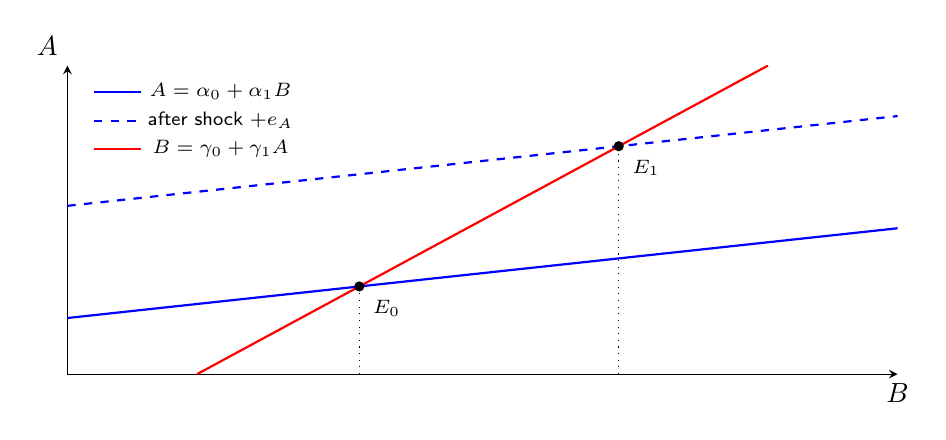
\begin{tikzpicture}
\begin{axis}[
  xlabel={$B$}, ylabel={$A$},
  xmin=0, xmax=3.2, ymin=0, ymax=5.5,
  axis lines=left,
  xtick=\empty, ytick=\empty,
  width=\textwidth, height=5.5cm,
  legend style={font=\scriptsize, at={(0.02,0.98)}, anchor=north west, draw=none, fill=none},
  every axis x label/.style={at={(axis description cs:1,0)}, anchor=north},
  every axis y label/.style={at={(axis description cs:0,1)}, anchor=south east}
]
\addplot[blue, thick, domain=0:3.2] {1 + 0.5*x};
\addlegendentry{$A=\alpha_0+\alpha_1 B$}
\addplot[blue, thick, dashed, domain=0:3.2] {3 + 0.5*x};
\addlegendentry{after shock $+e_A$}
\addplot[red, thick, domain=0.5:2.7] {(x - 0.5)/0.4};
\addlegendentry{$B=\gamma_0+\gamma_1 A$}
\node[circle, fill=black, inner sep=1.3pt, label={[font=\scriptsize]below right:$E_0$}] at (axis cs:1.125, 1.5625) {};
\node[circle, fill=black, inner sep=1.3pt, label={[font=\scriptsize]below right:$E_1$}] at (axis cs:2.125, 4.0625) {};
\draw[dotted] (axis cs:1.125, 0) -- (axis cs:1.125, 1.5625);
\draw[dotted] (axis cs:2.125, 0) -- (axis cs:2.125, 4.0625);
\end{axis}
\end{tikzpicture}
\end{column}
\begin{column}{0.45\textwidth}
\small
\begin{itemize}
\item $E_0$: equilibrium when $e_A=0$.
\item A positive shock $e_A$ shifts country A's reaction curve up.
\item New equilibrium $E_1$: \emph{both} $A$ \emph{and} $B$ rise.
\item Mechanism: $e_A\!\uparrow\,\Rightarrow A\!\uparrow\,\Rightarrow B\!\uparrow$ along B's reaction.
\item Same conclusion as the algebra: $\text{Cov}(B,e_A)=\frac{\gamma_1\sigma_A^2}{1-\gamma_1\alpha_1}>0$.
\end{itemize}
\end{column}
\end{columns}
\end{frame}


\begin{frame}{Endogeneity Source 3: Endogenous Choice (Selection)}
\begin{itemize}
\item Agents \textbf{choose} their treatment based on expected gains (Roy 1951).
\item Potential outcomes: $Y_i(1)=\bm{x}_i'\beta_1+e_{1i}$, \; $Y_i(0)=\bm{x}_i'\beta_0+e_{0i}$.
\item Selection rule: chooses treatment if net benefit exceeds threshold:
$$D_i = \mathbb{1}\{\bm{z}_i'\gamma + \eta_i > 0\}, \qquad \eta_i = e_{1i}-e_{0i}$$
\item Then $\eta_i$ is the \textbf{idiosyncratic gain} ($\tau_i = \bm{x}_i'(\beta_1{-}\beta_0)+\eta_i$); selecting on $\eta_i$ is \textbf{selection on gains}.
\item Mechanically $\text{Cov}(\eta_i,e_{1i})=\text{Var}(e_{1i})-\text{Cov}(e_{1i},e_{0i})\neq 0$, so
$$\mathbb{E}[e_{1i}\mid D_i=1]=\mathbb{E}[e_{1i}\mid \bm{z}_i'\gamma+\eta_i>0]\neq 0$$
and OLS on the treated sample is \alert{biased}.
\item If $\bm{z}$ includes variables excluded from $\bm{x}$, we have an \textbf{exclusion restriction}.
\end{itemize}
\end{frame}


\begin{frame}{Endogenous Choice: Political Selection}
\begin{itemize}
\item \textbf{Question:} Does holding office increase personal wealth?
$$\text{Wealth}_i = \beta_0 + \beta_1\;\text{HeldOffice}_i + \bm{x}_i'\gamma + e_i$$
\item Map to the framework: $D_i=\text{HeldOffice}_i$; $Y_i(1),Y_i(0)$ are wealth with/without office; $\eta_i$ is the idiosyncratic gain from holding office.
\item Problem: Who runs for office? Who wins?
\begin{itemize}
\item Wealthier individuals may be more likely to run and win
\item More politically connected individuals may both win and accumulate wealth
\item Selection on gains: those who expect to profit most from office seek it out
\end{itemize}
\item OLS recovers the observed difference, which mixes the causal effect with $\mathbb{E}[e_{1i}\mid D_i\!=\!1]\neq 0$:
$$\mathbb{E}[\text{Wealth}\mid D_i\!=\!1]-\mathbb{E}[\text{Wealth}\mid D_i\!=\!0] = \textcolor{blue}{\text{ATT}} + \textcolor{darkpurple}{\text{Selection bias}}$$
\end{itemize}
\end{frame}


\begin{frame}{Selection Bias Decomposition}
\begin{itemize}
\item The observed difference in outcomes:
\begin{multline*}
\mathbb{E}[Y\mid D\!=\!1]-\mathbb{E}[Y\mid D\!=\!0] = \underbrace{\mathbb{E}[Y(1)-Y(0)\mid D\!=\!1]}_{\text{ATT}}\\
 + \underbrace{\mathbb{E}[Y(0)\mid D\!=\!1]-\mathbb{E}[Y(0)\mid D\!=\!0]}_{\textcolor{darkpurple}{\text{Type I: Selection on levels}}}
\end{multline*}
\item If treatment effects are heterogeneous ($\tau_i = Y_i(1)-Y_i(0)$ varies):
$$\mathbb{E}[\tau_i\mid D=1]\neq \mathbb{E}[\tau_i] \quad\Rightarrow\quad \textcolor{blue}{\text{Type II: Selection on gains}}$$
\item \textbf{Type I:} Officeholders would have been wealthier anyway (baseline differences).
\item \textbf{Type II:} Those who gain most from office are most likely to seek it (differential returns).
\end{itemize}
\end{frame}


\begin{frame}{The Common Thread}
\begin{tcolorbox}[colback=blue!5, colframe=blue!50]
Measurement error, simultaneity, and selection all produce $\mathbb{E}[\bm{x}e]\neq 0$. IV identifies $\beta$ using an instrument $Z$.
\end{tcolorbox}
\vspace{0.3cm}
\begin{center}
\begin{tabular}{lll}
\toprule
\textbf{Source} & \textbf{Why $\mathbb{E}[\bm{x}e]\neq 0$} & \textbf{IV strategy}\\
\midrule
Measurement error & Noise in $\bm{x}$ enters error & Second measure of $\bm{x}^*$\\
Simultaneity & $Y$ and $X$ jointly determined & Exogenous shifter of one eq.\\
Selection/omitted var. & Choice correlated with $e$ & Exogenous shifter of choice\\
\bottomrule
\end{tabular}
\end{center}
\end{frame}


%%%%%%%%%%%%%%%%%%%%%%%%%%%%%%%%%%%%%%%%%%%%%%%%%%%
\section{IV Setup}
%%%%%%%%%%%%%%%%%%%%%%%%%%%%%%%%%%%%%%%%%%%%%%%%%%%

\begin{frame}{Notation: Structural Equation (Hansen Ch.\ 12)}
\begin{itemize}
\item $Y$ is a linear function of exogenous variables $\bm{x}_1$ and endogenous variables $\bm{y}_2$:
$$Y_1=\bm{x}_1'\beta_1+\bm{y}_2'\beta_2+e, \qquad \mathbb{E}[\bm{y}_2 e]\neq 0$$
\item \textbf{Instruments:} $\bm{z}=(\bm{z}_1', \bm{z}_2')'$, dimension $\ell\times 1$:
\begin{itemize}
\item $\bm{z}_1 = \bm{x}_1$: included instruments (the exogenous regressors), dimension $k_1$
\item $\bm{z}_2$: excluded instruments, dimension $\ell_2 \geq k_2$
\end{itemize}
\item Writing $\bm{x}=(\bm{x}_1', \bm{y}_2')'$ of dimension $k=k_1+k_2$:
$$Y_1 = \bm{x}'\beta + e$$
\end{itemize}
\end{frame}


\begin{frame}{Instrumental Variable Conditions}
\begin{tcolorbox}[colback=blue!5, colframe=blue!50]
\textbf{Three conditions} for valid instruments $\bm{z}$:
\begin{enumerate}
\item \textbf{Exogeneity:}  $\mathbb{E}[\bm{z}e]=0$ \quad (instrument uncorrelated with structural error)
\item \textbf{Relevance:}  $\text{rank}\;\mathbb{E}[\bm{z}\bm{x}']=k$ \quad (instruments predict endogenous regressors)
\item \textbf{Order condition:}  $\ell\geq k$ \quad (at least as many instruments as regressors)
\end{enumerate}
\end{tcolorbox}
\vspace{0.2cm}
\begin{itemize}
\item When $\ell=k$: \textbf{just identified} (exactly as many instruments as regressors)
\item When $\ell>k$: \textbf{overidentified} ($q=\ell-k$ overidentifying restrictions)
\item When $\ell<k$: \textbf{underidentified} (cannot estimate $\beta$)
\end{itemize}
\medskip
\small\alert{Aside.}\, \emph{Lagged values of the endogenous regressor are sometimes proposed as instruments.  Whether the exclusion restriction holds depends on the autocorrelation structure of the structural error --- developed in Lecture 18 (dynamic panels).}
\end{frame}


\begin{frame}{Causal Diagram for IV}
\begin{center}
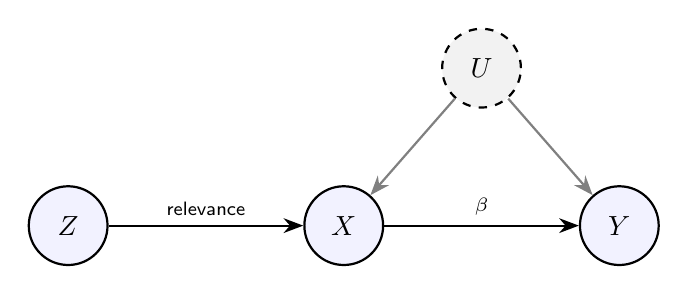
\begin{tikzpicture}[
  >={Stealth[length=2.5mm]},
  obs/.style={circle, draw, thick, minimum size=10mm, fill=blue!5},
  unobs/.style={circle, draw, thick, dashed, minimum size=10mm, fill=gray!10}
]
\node[obs] (Z) at (0,0) {$Z$};
\node[obs] (X) at (3.5,0) {$X$};
\node[obs] (Y) at (7,0) {$Y$};
\node[unobs] (U) at (5.25, 2) {$U$};

\draw[->, thick] (Z) -- node[above, font=\scriptsize]{relevance} (X);
\draw[->, thick] (X) -- node[above, font=\scriptsize]{$\beta$} (Y);
\draw[->, thick, gray] (U) -- (X);
\draw[->, thick, gray] (U) -- (Y);
\end{tikzpicture}
\end{center}

\vspace{0.1cm}
\small
\begin{itemize}
\item $U$ (dashed, unobserved): \textbf{confounder} of $X$ and $Y$; the source of $\mathbb{E}[Xe]\neq 0$.
\item \textbf{Relevance:} arrow $Z\to X$; the instrument moves the regressor.
\item \textbf{Exogeneity:} \emph{no} arrow $U\to Z$; the instrument is unconfounded.
\item \textbf{Exclusion:} \emph{no} direct arrow $Z\to Y$; $Z$ affects $Y$ \emph{only through} $X$.
\end{itemize}
\end{frame}


\begin{frame}{Example: Labeling the IV Setup}
\textbf{Do democratic institutions cause economic growth?} (Acemoglu, Johnson \& Robinson 2001)
\vspace{0.2cm}
\begin{itemize}
\item \textbf{Structural equation} ($Y_1 = \bm{x}_1'\beta_1 + \bm{y}_2'\beta_2 + e$):
$$\text{GDP/capita}_i = \beta_1\;\text{Latitude}_i + \beta_2\;\underbrace{\text{Institutions}_i}_{\bm{y}_2\text{: endogenous}} + e_i$$
\item \textbf{Endogeneity:} Richer countries may adopt better institutions (reverse causality); omitted factors (geography, culture) affect both.
\item \textbf{Excluded instrument} ($\bm{z}_2$): Colonial settler mortality.
\begin{itemize}
\item \textbf{Relevance:} High settler mortality $\Rightarrow$ extractive colonies $\Rightarrow$ weak institutions today.
\item \textbf{Exogeneity:} Historical disease environment affects current GDP only through institutions (exclusion restriction --- debatable!).
\end{itemize}
\end{itemize}
\end{frame}


%%%%%%%%%%%%%%%%%%%%%%%%%%%%%%%%%%%%%%%%%%%%%%%%%%%
\subsection{Reduced Form}
%%%%%%%%%%%%%%%%%%%%%%%%%%%%%%%%%%%%%%%%%%%%%%%%%%%

\begin{frame}{Why the Reduced Form?}
\begin{itemize}
\item OLS on the structural equation $Y_1 = \bm{x}'\beta + e$ is biased: $\mathbb{E}[\bm{x}e]\neq 0$.
\item But $\bm{z}$ is exogenous, so OLS \emph{regressions on $\bm{z}$} are consistent. Two are useful:
\begin{itemize}
\item \textbf{First stage:} project $\bm{y}_2$ on $\bm{z}$ to get coefficients $\Gamma$.
\item \textbf{Reduced form for $Y$:} project $Y_1$ on $\bm{z}$ to get coefficients $\lambda$.
\end{itemize}
\item These projections are tied to the structural $\beta$ via the map $\lambda = \bar{\Gamma}\beta$, where
$$\bar{\Gamma} = \mathbb{E}[\bm{z}\bm{z}']^{-1}\mathbb{E}[\bm{z}\bm{x}']$$
is the projection of the full regressor vector $\bm{x}=(\bm{x}_1', \bm{y}_2')'$ on $\bm{z}$.
\item \textbf{Plan:} estimate $\hat{\lambda}, \hat{\Gamma}$ by OLS, then recover $\beta$ by inverting $\lambda = \bar{\Gamma}\beta$.
\end{itemize}
\end{frame}


\begin{frame}{Reduced-Form Coefficients: Glossary}
\small
\begin{center}
\renewcommand{\arraystretch}{1.35}
\begin{tabular}{ll}
\toprule
\textbf{Symbol} & \textbf{Definition / role}\\
\midrule
$\Gamma$ & First stage: $\bm{y}_2 = \Gamma'\bm{z}+\bm{u}_2$, with $\Gamma = \mathbb{E}[\bm{z}\bm{z}']^{-1}\mathbb{E}[\bm{z}\bm{y}_2']$\\
$\Gamma_{12},\;\Gamma_{22}$ & Sub-blocks of $\Gamma$ on included ($\bm{z}_1$) / excluded ($\bm{z}_2$) instruments\\
$\bar{\Gamma}$ & Project full regressor $\bm{x}=(\bm{x}_1',\bm{y}_2')'$ on $\bm{z}$: $\;\bar{\Gamma}=\bigl[\begin{smallmatrix}\bm{I}_{k_1}&\Gamma_{12}\\ \bm{0}&\Gamma_{22}\end{smallmatrix}\bigr]$\\
$\lambda$ & Reduced form for $Y$: $\;Y_1 = \lambda'\bm{z}+u_1$, with $\lambda = \mathbb{E}[\bm{z}\bm{z}']^{-1}\mathbb{E}[\bm{z}Y_1]$\\
$\lambda_1,\;\lambda_2$ & Sub-blocks of $\lambda$ on $\bm{z}_1$ / $\bm{z}_2$\\
\bottomrule
\end{tabular}
\end{center}
\vspace{0.3cm}
\textbf{Key relation:} $\lambda = \bar{\Gamma}\beta$. Inverting this map recovers the structural $\beta$.
\end{frame}


\begin{frame}{Reduced Form: Definitions}
\begin{itemize}
\item Partition $\Gamma$ to match $\bm{z}=(\bm{z}_1', \bm{z}_2')'$:
$$\bm{y}_2 = \Gamma_{12}'\bm{z}_1+\Gamma_{22}'\bm{z}_2+\bm{u}_2, \qquad \Gamma = \begin{bmatrix}\Gamma_{12}\\ \Gamma_{22}\end{bmatrix}.$$
\begin{itemize}
\item $\Gamma_{12}$ ($k_1\times k_2$): coefficients on the included instruments $\bm{z}_1$.
\item $\Gamma_{22}$ ($\ell_2\times k_2$): coefficients on the excluded instruments $\bm{z}_2$.
\end{itemize}
\item Now project the full regressor vector $\bm{x}=(\bm{x}_1', \bm{y}_2')'$ on $\bm{z}$. Since $\bm{z}_1=\bm{x}_1$, the projection of $\bm{x}_1$ is $\bm{x}_1$ itself:
$$\bar{\Gamma} = \mathbb{E}[\bm{z}\bm{z}']^{-1}\mathbb{E}[\bm{z}\bm{x}'] = \begin{bmatrix} \bm{I}_{k_1} & \Gamma_{12}\\ \bm{0} & \Gamma_{22}\end{bmatrix}$$
\end{itemize}
\end{frame}


\begin{frame}{Reduced Form for $Y$}
\begin{itemize}
\item Substitute the reduced form for $\bm{y}_2$ into the structural equation (using $\bm{x}_1=\bm{z}_1$):
\begin{align*}
Y_1 &= \bm{z}_1'\beta_1 + (\Gamma_{12}'\bm{z}_1 + \Gamma_{22}'\bm{z}_2+\bm{u}_2)'\beta_2 + e\\
&= \bm{z}_1'\underbrace{(\beta_1+\Gamma_{12}\beta_2)}_{\lambda_1} + \bm{z}_2'\underbrace{\Gamma_{22}\beta_2}_{\lambda_2} + \underbrace{\bm{u}_2'\beta_2+e}_{u_1}
\end{align*}
\item The reduced-form error $u_1$ is orthogonal to $\bm{z}$ ($\mathbb{E}[\bm{z}u_1]=0$), so OLS consistently estimates $\lambda$.
\item Stacking: $\lambda = \bar{\Gamma}\beta$, which is just the matrix multiplication
$$\begin{bmatrix} \bm{I}_{k_1} & \Gamma_{12}\\ \bm{0} & \Gamma_{22}\end{bmatrix}\!\!\begin{bmatrix}\beta_1\\ \beta_2\end{bmatrix} = \begin{bmatrix}\beta_1+\Gamma_{12}\beta_2\\ \Gamma_{22}\beta_2\end{bmatrix}=\begin{bmatrix}\lambda_1\\ \lambda_2\end{bmatrix}$$
\item \textbf{Structural} parameters: $\beta_1,\beta_2$. \quad \textbf{Reduced-form} parameters: $\lambda, \Gamma$.
\end{itemize}
\end{frame}


\begin{frame}{Putting It Together}
\begin{itemize}
\item We now have two consistent OLS regressions:
\begin{itemize}
\item First stage: $\hat{\Gamma}\xrightarrow{p}\Gamma$
\item Reduced form for $Y$: $\hat{\lambda}\xrightarrow{p}\lambda$
\end{itemize}
\item Linked by the structural map $\lambda = \bar{\Gamma}\beta$: a system of $\ell$ linear equations in $k$ unknowns.
\item If $\bar{\Gamma}$ has rank $k$ (the \textbf{rank condition}), $\beta$ is uniquely pinned down by $\lambda$ and $\bar{\Gamma}$: the reduced form identifies the structural parameters.
\item Two cases follow:
\begin{itemize}
\item $\ell=k$ (just identified): invert the map, $\hat{\beta} = \bar{\hat{\Gamma}}^{-1}\hat{\lambda}$.
\item $\ell>k$ (overidentified): more equations than unknowns; need 2SLS to combine them.
\end{itemize}
\end{itemize}
\end{frame}


\begin{frame}{Reduced Form: The AJR Example}
\begin{itemize}
\item \textbf{Structural equation} (what we want):
$$\text{GDP}_i = \beta_1\;\text{Lat}_i + \beta_2\;\text{Institutions}_i + e_i$$
\item \textbf{First stage} (reduced form for $\bm{y}_2$):
$$\text{Institutions}_i = \underbrace{\Gamma_{12}}_{\text{Lat coeff}}\;\text{Lat}_i + \underbrace{\Gamma_{22}}_{\text{Mortality coeff}}\;\text{SettlerMort}_i + u_{2i}$$
\item \textbf{Reduced form for $Y$}:
$$\text{GDP}_i = \lambda_1\;\text{Lat}_i + \lambda_2\;\text{SettlerMort}_i + u_{1i}$$
\item \textbf{Invert the map} $\lambda = \bar{\Gamma}\beta$. With $\bar{\Gamma}$ upper-triangular, back-substitute:
$$\begin{bmatrix}\lambda_1\\ \lambda_2\end{bmatrix} = \begin{bmatrix} 1 & \Gamma_{12}\\ 0 & \Gamma_{22}\end{bmatrix}\begin{bmatrix}\beta_1\\ \beta_2\end{bmatrix} \;\Longrightarrow\; \beta_2 = \frac{\lambda_2}{\Gamma_{22}}, \;\; \beta_1 = \lambda_1 - \Gamma_{12}\beta_2.$$
\end{itemize}
\end{frame}


\begin{frame}{Identification}
\begin{itemize}
\item $\beta$ is \textbf{identified} if it is the unique solution to the moment conditions:
$$\mathbb{E}[\bm{z}(Y_1-\bm{x}'\beta)]=0$$
\item This is a system of $\ell$ equations in $k$ unknowns.
\item \textbf{Just identified} ($\ell=k$): unique solution $\beta = (\mathbb{E}[\bm{z}\bm{x}'])^{-1}\mathbb{E}[\bm{z}Y_1]$
\item Equivalently: if $\bar{\Gamma}$ has rank $k$, then $\beta=(\bar{\Gamma}'\bar{\Gamma})^{-1}\bar{\Gamma}'\lambda$.
\item \textbf{Overidentified} ($\ell>k$): system is overdetermined.
\begin{itemize}
\item No exact solution in general --- we need a method to combine the moment conditions.
\item \alert{Foreshadowing:} this is exactly the problem GMM solves (Lecture 15).
\end{itemize}
\item The \textbf{relevance condition} (rank $\mathbb{E}[\bm{z}\bm{x}']=k$) is what makes the solution exist.
\end{itemize}
\end{frame}


%%%%%%%%%%%%%%%%%%%%%%%%%%%%%%%%%%%%%%%%%%%%%%%%%%%
\section{The IV Estimator}
%%%%%%%%%%%%%%%%%%%%%%%%%%%%%%%%%%%%%%%%%%%%%%%%%%%

\begin{frame}{IV Estimator: Just-Identified Case}
\begin{itemize}
\item When $\ell=k$, the \textbf{IV estimator} is the sample analogue of the moment condition:
$$\hat{\beta}_{IV} = (Z'X)^{-1}Z'Y$$
\item Decompose:
\begin{align*}
\hat{\beta}_{IV} &= (Z'X)^{-1}Z'(X\beta+e)\\
&= \beta + (Z'X)^{-1}Z'e
\end{align*}
\item Consistency: $\text{plim}\;\hat{\beta}_{IV} = \beta + (E[ZX'])^{-1}E[Ze] = \beta$ \quad under exogeneity.
\end{itemize}
\end{frame}


\begin{frame}{Indirect Least Squares}
\begin{itemize}
\item \textbf{ILS}: Estimate reduced forms by OLS, then recover $\beta$.
\item Reduced form estimates:
$$\hat{\Gamma} = (Z'Z)^{-1}Z'X, \qquad \hat{\lambda} = (Z'Z)^{-1}Z'Y$$
\item When $\ell=k$: $\hat{\beta}_{ILS} = \hat{\Gamma}^{-1}\hat{\lambda}$
\item Show equivalence:
\begin{align*}
\hat{\beta}_{ILS} &= [(Z'Z)^{-1}Z'X]^{-1}(Z'Z)^{-1}Z'Y\\
&= (Z'X)^{-1}(Z'Z)(Z'Z)^{-1}Z'Y\\
&= (Z'X)^{-1}Z'Y = \hat{\beta}_{IV}
\end{align*}
\item ILS = IV in the just-identified case.
\end{itemize}
\end{frame}


\begin{frame}{The Wald Estimator}
\begin{itemize}
\item Special case: single endogenous $X$, single binary instrument $Z\in\{0,1\}$.
\item The IV estimator simplifies to the \textbf{Wald estimator}:
$$\hat{\beta}_{Wald} = \frac{\bar{Y}_{Z=1}-\bar{Y}_{Z=0}}{\bar{X}_{Z=1}-\bar{X}_{Z=0}} = \frac{\text{Reduced form effect on } Y}{\text{First stage effect on } X}$$
\item Intuition: scale the \textbf{intent-to-treat} (ITT) effect by the first-stage compliance rate.
\item This is a ratio of two consistent estimators --- a \textbf{ratio estimator}.
\item \textbf{Canonical setting:} \textbf{randomized binary encouragement designs}. $Z$ is randomly assigned (lottery, mailing, eligibility); $X$ is binary take-up. Random assignment delivers exogeneity; the first stage measures compliance. The draft lottery (next slide) is a textbook example.
\end{itemize}
\end{frame}


\begin{frame}{Wald Estimator: Draft Lottery and Civic Participation}
\begin{itemize}
\item \textbf{Question:} Does military service increase political participation?
\item $Y$ = voter turnout, $X$ = served in military, $Z$ = draft lottery number (low = drafted).
\item \textbf{Reduced form:} $\bar{Y}_{Z=\text{low}} - \bar{Y}_{Z=\text{high}}$ = effect of lottery on turnout (ITT).
\item \textbf{First stage:} $\bar{X}_{Z=\text{low}} - \bar{X}_{Z=\text{high}}$ = effect of lottery on service rate.
$$\hat{\beta}_{Wald} = \frac{\text{ITT on turnout}}{\text{First stage compliance}} = \frac{\text{Reduced form}}{\text{First stage}}$$
\item Not everyone drafted actually serves (deferments, exemptions).
\item The Wald estimator rescales the ITT by the share who comply with the draft.
\end{itemize}
\end{frame}


%%%%%%%%%%%%%%%%%%%%%%%%%%%%%%%%%%%%%%%%%%%%%%%%%%%
\section{2SLS}
%%%%%%%%%%%%%%%%%%%%%%%%%%%%%%%%%%%%%%%%%%%%%%%%%%%

\begin{frame}{Two-Stage Least Squares}
\begin{itemize}
\item When $\ell>k$ (overidentified), we need 2SLS.
\item \textbf{Stage 1:}  Regress $X$ on $Z$:
$$\hat{X} = P_Z X, \qquad P_Z = Z(Z'Z)^{-1}Z'$$
\item \textbf{Stage 2:}  Regress $Y$ on $\hat{X}$:
$$\hat{\beta}_{2SLS} = (\hat{X}'\hat{X})^{-1}\hat{X}'Y = (X'P_ZX)^{-1}X'P_ZY$$
\item The projection $P_Z$ extracts the \textbf{exogenous variation} in $X$ --- the part predicted by instruments.
\end{itemize}
\end{frame}


\begin{frame}{2SLS = IV When Just Identified}
\begin{itemize}
\item When $\ell=k$, $P_Z = Z(Z'Z)^{-1}Z'$ and:
\begin{align*}
\hat{\beta}_{2SLS}&=(\hat{X}'\hat{X})^{-1}\hat{X}'Y\\
&=(X'P_ZX)^{-1}X'P_ZY\\
&=(X'Z(Z'Z)^{-1}Z'X)^{-1}X'Z(Z'Z)^{-1}Z'Y\\
&=(Z'X)^{-1}(Z'Z)(X'Z)^{-1}X'Z(Z'Z)^{-1}Z'Y \tag{$(ABC)^{-1}=C^{-1}B^{-1}A^{-1}$}\\
&=(Z'X)^{-1}Z'Y = \hat{\beta}_{IV}
\end{align*}
\item 2SLS generalizes IV to the overidentified case.
\end{itemize}
\end{frame}


\begin{frame}[fragile]{R Implementation}
\begin{lstlisting}
library(estimatr)

# 2SLS estimation
# Y ~ endogenous + exogenous | excluded_instruments + exogenous
fit_iv <- iv_robust(Y ~ D + X | Z + X, data = dat)
summary(fit_iv)
\end{lstlisting}
\begin{itemize}
\item Variables before ``\textbar'' are the structural equation regressors.
\item Variables after ``\textbar'' are the instruments (excluded + included).
\item \texttt{iv\_robust} uses heteroskedasticity-robust standard errors by default.
\end{itemize}
\end{frame}


\begin{frame}{Why Discuss ILS?}
\begin{itemize}
\item In modern practice, 2SLS dominates: it works for any $\ell\geq k$ and reduces to ILS when $\ell=k$.
\item ILS is a throwback to the \textbf{Cowles Commission} (1940s--50s; Haavelmo, Koopmans, Marschak, Theil) and its \textbf{simultaneous-equations} worldview.
\item That framework was built for systems where many things are jointly determined:
\begin{itemize}
\item \textbf{Supply and demand:} $p,q$ pinned down at the intersection; supply shifters identify demand, demand shifters identify supply.
\item \textbf{Strategic interaction:} best responses depend on rivals' choices (Cournot, Stackelberg).
\item \textbf{Macro feedback:} consumption $\leftrightarrow$ income, investment $\leftrightarrow$ output.
\end{itemize}
\item The Angrist-Imbens revolution shifted IV practice toward single endogenous regressors with quasi-experimental instruments. The vocabulary (``first stage,'' ``reduced form,'' ``identification'') is inherited from Cowles; the multi-equation machinery has mostly receded.
\end{itemize}
\end{frame}


\begin{frame}{Real-World Instruments: Four Common Sources}
\begin{enumerate}
\item \textbf{Experimental assignment with imperfect compliance.} Random offer of treatment (canvassing, voucher, training) when take-up is incomplete. Ex: Gerber \& Green GOTV mailings (assigned $\to$ contacted $\to$ turnout); MTO housing vouchers.
\item \textbf{Explicit administrative random assignment.} Lotteries and random bureaucratic processes. Ex: Vietnam draft lottery (Angrist 1990); reservation of village council seats for women (Chattopadhyay \& Duflo 2004); random assignment of cases to judges (Aizer \& Doyle 2015).
\item \textbf{Weather fluctuations and global price shocks.} Local economic conditions move with exogenous external forces. Ex: rainfall and civil war (Miguel, Satyanath, Sergenti 2004); commodity-price shocks and conflict (Brückner \& Ciccone 2010; Bazzi \& Blattman 2014).
\item \textbf{Bartik / shift-share instruments.} National sectoral shocks $\times$ predetermined local exposure shares. Ex: China import shock (Autor, Dorn, Hanson 2013) $\to$ local import competition $\to$ wages, vote polarization.
\end{enumerate}
\end{frame}


\begin{frame}{Real-World Instruments (continued)}
\begin{enumerate}\setcounter{enumi}{4}
\item \textbf{Nonrandom thresholds on running variables (RD as IV).} An arbitrary cutoff of a continuous covariate flips treatment status; near the threshold the running variable acts as an instrument.
\begin{itemize}
\item Population thresholds triggering mayoral powers, fiscal rules, or council size (Pettersson-Lidbom 2012 on Swedish municipalities; Italian and Brazilian municipal studies).
\item Arbitrary eligibility cutoffs for resource allocation: IRA tax-credit thresholds (Zikai Li); Title I funding; Maimonides' rule for class size (Angrist \& Lavy 1999).
\end{itemize}
\item \textbf{Technology rollouts shaped by preexisting geography.} A new technology diffuses according to terrain or infrastructure that predates the outcome of interest, so reception is exogenous to it.
\begin{itemize}
\item Broadcast signal strength at the advent of radio/TV: Yanagizawa-Drott (2014) on Rwandan radio and genocide; DellaVigna et al.\ (2014) on Serbian TV in Croatia; Adena et al.\ (2015) on radio and the rise of the Nazis.
\end{itemize}
\end{enumerate}
\end{frame}


%%%%%%%%%%%%%%%%%%%%%%%%%%%%%%%%%%%%%%%%%%%%%%%%%%%
\section{Asymptotic Theory}
%%%%%%%%%%%%%%%%%%%%%%%%%%%%%%%%%%%%%%%%%%%%%%%%%%%

\begin{frame}{Consistency of 2SLS (Hansen Thm.\ 12.1)}
\begin{thm}[Consistency]
Under the conditions: (1) $E[Ze]=0$, (2) $\text{rank}\;E[ZX']=k$, (3) $E[ZZ']>0$, the 2SLS estimator is consistent: $\hat{\beta}_{2SLS}\xrightarrow{p}\beta$.
\end{thm}
\vspace{0.2cm}
\textbf{Proof sketch:}
$$\hat{\beta}_{2SLS}-\beta = \left(\frac{X'P_ZX}{n}\right)^{-1}\frac{X'P_Ze}{n}$$
Define $Q_{XZ}=E[XZ']$, $Q_{ZZ}=E[ZZ']$, $Q_{ZX}=E[ZX']$.  Then:
$$\xrightarrow{p}\; (Q_{XZ}Q_{ZZ}^{-1}Q_{ZX})^{-1}Q_{XZ}Q_{ZZ}^{-1}\underbrace{E[Z'e]}_{=0} = 0$$
\end{frame}


\begin{frame}{Just-Identified IV: Asymptotic Distribution}
\begin{itemize}
\item For just-identified IV ($\ell=k$), $\hat{\beta}_{IV}=(Z'X)^{-1}Z'Y$, and
$$\sqrt{n}(\hat{\beta}_{IV}-\beta) = \left(\frac{Z'X}{n}\right)^{-1}\frac{Z'e}{\sqrt{n}}.$$
\item WLLN: $\dfrac{Z'X}{n}\xrightarrow{p}Q\equiv\mathbb{E}[\bm{z}\bm{x}']$ ($k\times k$ since $\ell=k$).
\item CLT: $\dfrac{Z'e}{\sqrt{n}}\xrightarrow{d} N(0,\Omega)$, $\Omega\equiv\mathbb{E}[\bm{z}\bm{z}'e^2]$.
\item Slutsky:
\end{itemize}
\begin{tcolorbox}[colback=blue!5, colframe=blue!50]
$$\sqrt{n}(\hat{\beta}_{IV}-\beta)\xrightarrow{d} N\!\left(0,\;Q^{-1}\Omega\, Q^{-1\prime}\right).$$
\end{tcolorbox}
The general 2SLS sandwich (next slide) reduces to this when $\ell=k$.
\end{frame}


\begin{frame}{Asymptotic Distribution (Hansen Thm.\ 12.2)}
\begin{thm}[Asymptotic Normality]
Under regularity conditions:
$$\sqrt{n}(\hat{\beta}_{2SLS}-\beta)\xrightarrow{d} N(0, V_\beta)$$
where:
$$V_\beta = (Q_{XZ}Q_{ZZ}^{-1}Q_{ZX})^{-1}Q_{XZ}Q_{ZZ}^{-1}\Omega Q_{ZZ}^{-1}Q_{ZX}(Q_{XZ}Q_{ZZ}^{-1}Q_{ZX})^{-1}$$
with $Q_{XZ}=E[\bm{x}_i\bm{z}_i']$, $Q_{ZZ}=E[\bm{z}_i\bm{z}_i']$, $Q_{ZX}=E[\bm{z}_i\bm{x}_i']$, $\Omega=E[\bm{z}_i\bm{z}_i'e_i^2]$.
\end{thm}
\begin{itemize}
\item Under homoskedasticity ($E[e^2\mid Z]=\sigma^2$), this simplifies to:
$$V_\beta = \sigma^2(Q_{XZ}Q_{ZZ}^{-1}Q_{ZX})^{-1}$$
\item Under heteroskedasticity, use robust covariance estimation (as in Lecture 8).
\end{itemize}
\end{frame}


\begin{frame}{Sample Analogs: Plug-in Variance for Just-Identified IV}
\begin{itemize}
\item Replace population moments with sample averages.  Form residuals $\hat{e}_i = Y_i - \bm{x}_i'\hat{\beta}_{IV}$ (using the original $\bm{x}_i$, not $\hat{\bm{x}}_i$).
\item Sample analogs:
$$\hat{Q}=\frac{1}{n}\sum_{i=1}^n \bm{z}_i\bm{x}_i', \qquad \hat{\Omega}=\frac{1}{n}\sum_{i=1}^n \bm{z}_i\bm{z}_i'\hat{e}_i^2.$$
\end{itemize}
\begin{tcolorbox}[colback=blue!5, colframe=blue!50]
$$\widehat{\text{Var}}(\hat{\beta}_{IV})=\frac{1}{n}\,\hat{Q}^{-1}\hat{\Omega}\,\hat{Q}^{-1\prime}$$
\end{tcolorbox}
\begin{itemize}
\item \textbf{What you do with data:} compute $\hat{Q}$ as a matrix of cross-products, compute residuals, compute $\hat{\Omega}$ as a $z\bar{z}'$-weighted average of squared residuals, sandwich them.
\item Under conditional homoskedasticity $\hat{\Omega}=\hat{\sigma}^2\,\hat{Q}_{ZZ}$, recovering the classical formula.
\end{itemize}
\end{frame}


\begin{frame}{Variance Estimation: 2SLS}
\begin{itemize}
\item \textbf{Homoskedastic} variance estimator:
$$\hat{V}_\beta = \hat{\sigma}^2(X'P_ZX)^{-1}, \qquad \hat{\sigma}^2 = \frac{\hat{e}'\hat{e}}{n-k}$$
where $\hat{e}=Y-X\hat{\beta}_{2SLS}$ (use \textbf{original} $X$, not $\hat{X}$).
\item \textbf{Heteroskedastic-robust} (analogous to HC):
$$\hat{V}_\beta = (X'P_ZX)^{-1}\left(\sum_{i=1}^n \hat{e}_i^2 \hat{X}_i\hat{X}_i'\right)(X'P_ZX)^{-1}$$
\item \alert{Important:} Standard errors from the ``naive'' second-stage regression (regressing $Y$ on $\hat{X}$ and reading off SEs) are \textbf{incorrect} --- they use $\hat{X}$ instead of $X$ in the residuals.
\end{itemize}
\end{frame}


\begin{frame}{Wald Tests with IV/2SLS}
\begin{itemize}
\item To test the linear restriction $H_0:\bm{R}\beta=\bm{r}$ ($q$ restrictions), form
$$W_n = n(\bm{R}\hat{\beta}-\bm{r})'\bigl(\bm{R}\,\hat{V}\,\bm{R}'\bigr)^{-1}(\bm{R}\hat{\beta}-\bm{r})\xrightarrow{d}\chi^2_q,$$
where $\hat{V}=\hat{Q}^{-1}\hat{\Omega}\hat{Q}^{-1\prime}$ (just-identified) or the 2SLS sandwich (overidentified).
\item Reject $H_0$ at level $\alpha$ if $W_n>\chi^2_{q,1-\alpha}$.  For a single coefficient: $t=\sqrt{W_n}$, compare to $\pm 1.96$.
\end{itemize}
\medskip
\textbf{Example: equality of IV slopes across two independent samples.}
\begin{itemize}
\item Sample 1 (e.g., women), sample 2 (e.g., men), each just identified, separate $\hat{\beta}_j$, $\hat{V}_j$.
\item Independence (different individuals) $\Rightarrow \hat{\beta}_1\perp\hat{\beta}_2$ asymptotically.
\item Test $H_0:\beta_1=\beta_2$ via
$$W_n = n(\hat{\beta}_1-\hat{\beta}_2)'\bigl(\hat{V}_1+\hat{V}_2\bigr)^{-1}(\hat{\beta}_1-\hat{\beta}_2)\xrightarrow{d}\chi^2_k.$$
\end{itemize}
\end{frame}


%%%%%%%%%%%%%%%%%%%%%%%%%%%%%%%%%%%%%%%%%%%%%%%%%%%
\section{Moment Conditions and GMM Preview}
%%%%%%%%%%%%%%%%%%%%%%%%%%%%%%%%%%%%%%%%%%%%%%%%%%%

\begin{frame}{IV as a Method of Moments}
\begin{itemize}
\item The IV estimator solves the \textbf{sample moment condition}:
$$\frac{1}{n}\sum_{i=1}^n Z_i(Y_i - X_i'\beta) = 0$$
\item This is a system of $\ell$ equations in $k$ unknowns.
\item When $\ell=k$: exactly identified, unique solution.
\item When $\ell>k$: overidentified, no exact solution.
\item \textbf{2SLS resolves this} by using a specific weighting matrix:
$$\hat{\beta}_{2SLS} = \arg\min_\beta \left[\frac{1}{n}\sum Z_i(Y_i-X_i'\beta)\right]'(Z'Z/n)^{-1}\left[\frac{1}{n}\sum Z_i(Y_i-X_i'\beta)\right]$$
\end{itemize}
\end{frame}


\begin{frame}{IV Through the Theory-to-Moment Workflow}
Recall the workflow from Lecture 6:

\medskip
\begin{enumerate}
\item \textbf{Mechanism:} $X$ causes $Y$, but $X$ is endogenous ($\mathbb{E}[X_i e_i]\neq 0$).
\item \textbf{Exogenous feature:} An instrument $Z$ is independent of $e$ by institutional design, randomization, or natural experiment.
\item \textbf{Observable implication:} $Z$ predicts $X$ but is uncorrelated with the structural error.
\item \textbf{Moment condition:} $\mathbb{E}[Z_i(Y_i - X_i'\beta)]=0$\quad (replacing $X_i$ with $Z_i$).
\item \textbf{Estimator:} $\hat{\beta}_{IV}=(Z'X)^{-1}Z'Y$.
\end{enumerate}
\end{frame}


\begin{frame}{Foreshadowing GMM}
\begin{itemize}
\item 2SLS uses the weighting matrix $\hat{W}=(Z'Z/n)^{-1}$.
\item Is this the \textbf{optimal} weighting?
\begin{itemize}
\item Under homoskedasticity: \textbf{yes}.
\item Under heteroskedasticity: \textbf{no} --- there exists a more efficient choice.
\end{itemize}
\item The \textbf{Generalized Method of Moments} (GMM) chooses $\hat{W}$ optimally:
$$\hat{W}_{opt} = \hat{\Omega}^{-1}, \qquad \hat{\Omega} = \frac{1}{n}\sum_{i=1}^n \hat{e}_i^2 Z_iZ_i'$$
\item GMM also extends beyond linear IV to \textbf{any} set of moment conditions.
\item \alert{Next week:} we develop the full GMM framework.
\end{itemize}
\end{frame}


\begin{frame}{Summary}
\begin{enumerate}
\item Endogeneity ($E[Xe]\neq 0$) makes OLS inconsistent for structural parameters.
\item Instruments $Z$ satisfying exogeneity and relevance allow consistent estimation.
\item The IV estimator $\hat{\beta}_{IV}=(Z'X)^{-1}Z'Y$ works when just identified.
\item 2SLS $\hat{\beta}_{2SLS}=(X'P_ZX)^{-1}X'P_ZY$ generalizes to overidentification.
\item Both are consistent and asymptotically normal under standard conditions.
\item IV is a \textbf{method of moments} --- 2SLS is a specific weighting of moment conditions.
\end{enumerate}
\vspace{0.2cm}
\begin{tcolorbox}[colback=blue!5, colframe=blue!50]
\textbf{Next lecture:} Finite sample properties, testing, LATE, and the MTE framework.
\end{tcolorbox}
\end{frame}

\end{document}
